\documentclass[10pt,twocolumn,letterpaper]{article}

\usepackage{statcourse}
\usepackage{times}
\usepackage{epsfig}
\usepackage{graphicx}
\usepackage{amsmath}
\usepackage{amssymb}

% Include other packages here, before hyperref.

% If you comment hyperref and then uncomment it, you should delete
% egpaper.aux before re-running latex.  (Or just hit 'q' on the first latex
% run, let it finish, and you should be clear).
\usepackage[breaklinks=true,bookmarks=false]{hyperref}


\statcoursefinalcopy


\setcounter{page}{1}
\begin{document}


%%%%%%%%%%%%%%%%%%%%%%%%%%%%%%%%%%%%%%%%%%%%%%%%%%%%%%%%%%%%%%%
% DO NOT EDIT ANYTHING ABOVE THIS LINE
% EXCEPT IF YOU LIKE TO USE ADDITIONAL PACKAGES
%%%%%%%%%%%%%%%%%%%%%%%%%%%%%%%%%%%%%%%%%%%%%%%%%%%%%%%%%%%%%%%



%%%%%%%%% TITLE
\title{Comparative Analysis of Machine Learning Models: \\Alexnet, VGG, Resnet, YOLO}

\author{Pham Duc An\\
{\tt\small 10422002}
\and
Tran Hai Duong\\
{\tt\small 10422021}
\and
Vo Thi Hong Ha\\
{\tt\small 10421015}
\and
Nguyen Hoang Anh Khoa\\
{\tt\small 10422037}
\and
Truong Hao Nhien\\
{\tt\small 10422062}
\and
Nguyen Song Thien Phuc\\
{\tt\small 10422067}\\
\\
\{\tt @student.vgu.edu.vn\}
\and
Bui Duc Xuan\\
{\tt\small 10422085}
}

\maketitle
%\thispagestyle{empty}



% MAIN ARTICLE GOES BELOW
%%%%%%%%%%%%%%%%%%%%%%%%%%%%%%%%%%%%%%%%%%%%%%%%%%%%%%%%%%%%%%%


%%%%%%%%% ABSTRACT
\begin{abstract}
   In this project, we conducted a comprehensive comparative analysis of prominent machine learning models, namely Alexnet, VGG, Resnet, and YOLO, with a focus on their efficacy in image recognition. Leveraging a curated dataset representative of diverse real-world scenarios with CIFAR-10, our study delved into the nuances of each model's architecture, training process, and computational requirements. Through rigorous evaluation using metrics such as accuracy, precision, and recall, our results reveal nuanced performance distinctions. Notably, Resnet demonstrated superior accuracy, VGG excelled in feature extraction, YOLO showcased real-time efficiency, and Alexnet exhibited a stable performance. These findings provide valuable insights for practitioners and researchers seeking to optimize model selection for specific applications, shedding light on the trade-offs between accuracy, computational cost, and real-time processing capabilities. Project's detailed code are provided at {\url{https://github.com/nhientruong04/LIA-introCS-proj}}.
\end{abstract}

%%%%%%%%% BODY TEXT
\section{Models}

\subsection{VGGNet}
\subsubsection{The motivation behind the VGGNet Model}
The VGGNet model, officially known as the OxfordNet, was introduced in the paper titled 
“ Very Deep Convolutional Networks for Large-Scale Image Recognition”, presented at the 
International Conference on Learning Representations (ICLR) in 2015. The VGGNet achieved 
notable success in the ImageNet Large Scale Visual  Recognition Challenge (ILSVRC) in 2014, 
showcasing the model’s mobility to excel in large-scale image classification tasks. In particular, 
it achieved a test accuracy of 92.7 percent in ImageNet, a dataset containing more than 14 million 
training images across 1000 object classes, paving the way for subsequent research in deep learning 
and inspiring the exploration of even deeper neural network architectures.
\subsubsection{Architecture}
\paragraph{Deep Dark Fantasy}
The general architecture of the VGGNet model is much deeper in comparison to that of AlexNet, which 
was a significant advancement at the time of its creation. One of its variants is VGG16 consists of 
16 weight layers including 13 convolutional layers, and 3 fully-connected layers, with a total of 138 
million parameters.\cite{tammina2019transfer} This depth is beneficial for its hierarchical feature 
learning. Deeper networks can learn robust and discriminative representations of features. Each layer 
in the network can capture increasingly abstract and complex features. This hierarchy allows the network 
to understand patterns at multiple levels of granularity. Another variant of VGGNet is VGG19, which has 
the similar structure of VGG16, except for the insertion of three more convolutional layers. In general, 
while maintaining the same structure and size of fully connected layers, VGG19 is deeper than VGG16 with 
19 layers, potentially capturing more intricate features from images. Moreover, with more layers, VGG19 is 
computationally more intensive both in terms of memory and processing power compared to VGG16, but it does 
not indicate that there is a significant difference in the output of these models. The performance improvements 
gained by utilizing two VGGNet variants are marginal, especially in scenarios where training data might not be 
extensive enough to fully leverage the deeper architecture.\\

Furthermore, the pre-trained VGG16 model can be fine-tuned for various tasks, which refers to the process of 
taking a pre-trained neural network and further training it on a new dataset or for a specific task, also known 
as transfer learning. In this case, the VGGNet models,including two variants VGG16 and VGG19, are already trained 
on ImageNet, which comprises over 14 million training images with thousands of disparate categories. Trained on huge 
datasets, the model has learned a good representation of low level features such as spatial, edges, rotation, lightning, 
shapes and these features can be shared across to enable the knowledge be leveraged and act as a feature extractor for 
new images in different computer vision problems based on the principles of transfer learning, even when the new images 
are of completely different categories from the source dataset.

\begin{figure}
\begin{center}
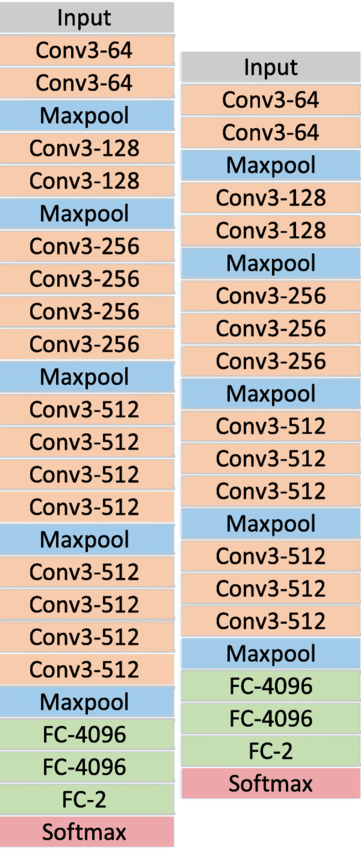
\includegraphics[width=0.4\textwidth]
{figures/VGG_arc_compare.png}
 \caption{The architecture of VGG19 and VGG16.}
 \label{fig:picture}
\end{center}
\end{figure}

\paragraph{Stacks of Smaller Convolutional Filters}
Rather than using relatively large receptive fields in the  first convolutional layers, multiple tiny 3x3 receptive 
fields are selected throughout the whole net, which are convolved with the input at every pixel with a stride of 1. 
The presented figures delineate that a stack of two 3x3 convolutional layers has an effective receptive field of 5x5. 
Hence, it can be concluded that a stack of three 3x3 convolutional filters has an effective receptive field of 7x7.\\
Assuming it is obvious that stacks of small-kernel convolution layers have equal sized receptive fields, what makes them 
a more optimal choice? The initial point is incorporating more rectification layers instead of s single one, on the grounds 
that more non-linear activation layers accompany the convolutional layers,  reducing the network’s tendency to over-fit during 
training exercises, improving the decision functions and allowing the network to converge quickly. In addition, with a small 
receptive field, a stack of 3x3 convolution filters have fewer parameters to train,\cite{simonyan2015deep} saving computational 
resources needed for training and inference, hence offering lower computational complexity.

\section{Challenges}
During the project, it is inevitable that we encounter multifaceted challenges, since AI research has never been effortless. 
With regards to experience, almost all of the members had never approached the concept of machine learning in general and computer 
vision in particular. It was necessary for us to read scientific papers, while each member had little opportunity and experience 
to get used to reading journals. Hence, this procedure was so demanding, owing to the overwhelming number of journals of numerous 
subjects; and at the same time, we lacked the orientation towards selecting appropriate articles for the required domain knowledge 
in computer vision. Furthermore, this project involves interdisciplinary aspects where a lack of in-depth knowledge in certain domains 
presented challenges, especially Linear Algebra. On the grounds that it plays a fundamental role in the field of Convolutional Neural 
Networks, we were required to have a concrete foundation in some aspects of this discipline and apply them in computer vision tasks. 
For instance, comprehending matrix operations demystifies the techniques and processes inside the convolutional and pooling layers; 
or tensor representations simplify input handling, as when images are viewed as tensors, it is much easier to understand how CNNs 
process data. In addition to this, a lack of resources serving for training purposes also hindered the project. Specifically, the 
lack of powerful and reliable GPUs to train all chosen models and their variants necessitated more time. Ultimately, the project 
operated under stringent time constraints due to the abundance of time spent on reading papers and acquiring sufficient knowledge 
to build four selected AI models. The initial project schedule, carefully crafted to allow for comprehensive testing and logging 
the results to compare the performance of them, was significantly compressed to meet the accelerated product launch timeline. However, 
some procrastinations arose during the timeframe,  given that the time spent on researching was considerable and the time-consuming 
process of training four models made the stage of logging and comparing metrics prolonged.
{\small
\bibliographystyle{ieee}
\bibliography{bibliography.bib}
}

\end{document}